\chapter{Introduction: Diffeomorphisms in Medical Imaging Registration}\label{ch:introduction}


\begin{flushright}
		\emph{The series is divergent, therefore we may be able \\ to do something with it.}\\
			- Oliver Heaviside
\end{flushright}

\vspace{0.6cm}


Aim of this chapter is to introduce the log-composition. It arises in medical image registration, when diffeomorphisms are utilized to model the transformation of anatomies between images. Before getting into it formalization, it is important to spend some few words about the context and the reasons that led to this definition. 

\section{Toward an ill-posed Problem}
Medical image registration is a set of tools and techniques oriented to solve the problem of determining correspondences between two or more images acquired from patients scans. Its development is a creative field that has seen the application of a growing number of mathematical theories in the research of customizations and improvements.

Involved difficulties and opportunities are a consequence of the fact that dealing with image registration problem means dealing with an ill-posed problem. Transformations between anatomies are not unique, and the impossibility to recover spatial or temporal evolution of an anatomical transformation from temporally isolated images, makes any validation a difficult, if not an impossible task. 
In addition each situation inevitably brings some prior knowledge within the initial data, that may imply some modifications in the problems' setting and may imply some additional constraints. This, of course, impacts dramatically the range of possible choices in searching for a solution and in the consequent results. 

Certainly it is the practical situation that provides the hint in choosing the optimal constraints, but it almost never provides enough information to reduce the large amount of options involved. A wide range of variants in methodologies and approaches to solve the registration problem has been thus proposed in the last decades: a quick glance to Google scholar reveals about $1200000$ papers in \emph{medical image registration} (55\% of the whole \emph{image registration} resources). 

\subsection{Some Examples of Medical Image Registration}
One of the most studied application of image registration is in the domain of brain imaging: there this tool can be used to examine differences between subjects and distinguish their biological features - cross-sectional studies - or to compare different acquisition of the same subject after a fixed period of time or before and after a surgical operation - longitudinal studies. 

In both cross-sectional and longitudinal studies an accurate comparison between images and the parameters of the transformation involved may result in a quantification of anatomical variability and in a better understanding of the patients' features. 
%
For example, brain atrophy is considered a biomarker to diagnose Alzheimer disease and to analyze its evolution; most of the algorithms and techniques involved in the atrophy measurement require longitudinal or cross-sectional scans to be aligned, and so are directly affected by the solution of the registration algorithm \cite{prados2015measuring}, \cite{fox1997brain}, \cite{gauthier2012prevention}. 

Also when dealing with motion correction, if a sequence of images is affected by the motion of cardiac pulses or respiratory cycles, registration algorithms are often used for the realignment. 
For example, in lungs radiotherapy, the correspondence between the lungs' deformation and the respiratory signal defines a model to direct the X-ray or electrons beam on the cancer, avoiding as much as possible the sane tissue. Lungs deformation is obtained using a registration algorithms that provides the direction of the motion of each voxel in each phase of breathing \cite{mcclelland}, \cite{mcclelland2011inter}.

Another application of image registration is the operation of gluing together several pictures with partially coincident regions, with the aim of obtaining a bigger image of the whole scene. This procedure, called \emph{mosaicing}, exploit registration algorithms to aligns images using information obtained form the overlapping regions \cite{vercauteren2006robust}, \cite{szeliski1994image}.

The next section moves toward some details of one iterative framework most commonly utilized by image registration algorithms.

% % % % % % % % % % % % % % % % % % % % % % % % % % % % % % % % % % % % % %
% % SUBSECTION
% % % % % % % % % % % % % % % % % % % % % % % % % % % % % % % % % % % % % %

\subsection{Image Registration Problem}\label{se:registration_framework}

A \emph{$d$-dimensional image} is a continuous function from a subset $\Omega$ of the coordinate space $\mathbb{R}^{d}$ (having in mind particular cases $d=2,3$) to the set of real numbers $\mathbb{R}$. Given two of them, $F : \Omega_{F}  \rightarrow\mathbb{R} $ and $M : \Omega_{M}  \rightarrow\mathbb{R} $, called respectively \emph{fixed image} and \emph{moving image}, the \emph{image registration problem} consists in finding the transformation function
\begin{align*}
\varphi :\mathbb{R}^{d} \supseteq \Omega_{F} & \longrightarrow \Omega_{M}\subseteq \mathbb{R}^{d}   \\
\mathbf{x} &\longmapsto \varphi (\mathbf{x}) 
\end{align*}
such that for each point $\mathbf{x}\in \Omega_{F} $ the element $M(\varphi (\mathbf{x}))$ and $F(\mathbf{x})$ are as closed as possible according to a chosen measure of similarity. Other than obtaining $\varphi$, also the investigation of its features and parameters are a part of the problem.

The definition of image registration problem proposed here can be represented by the following diagram, where $\varphi$ is the solution that, in the ideal case, makes $f$ the function that match the correspondences in the intensities when images are aligned:

\[
\begindc{\commdiag}[40]
\obj(-30,30)[Or]{$\Omega_{F}$}
\obj(0,30)[Ot]{$\Omega_{M}$}
\obj(-30,10)[Rref]{$\mathbb{R}$}
\obj(0,10)[Rtarg]{$\mathbb{R}$}

\mor{Or}{Ot}{$\varphi$}
\mor{Or}{Rref}{$F$}
\mor{Ot}{Rtarg}{$M$}
\mor{Rref}{Rtarg}{f}[1,1]

\enddc
\]
% fine diagramma
\noindent
The composition of the moving image after the transformation, $M\circ\varphi $, is called \emph{warped image}, and
if $\Omega_{F} \neq \Omega_{M}$, it is always possible to apply an homeomorphism to transform them into a common domain $\Omega$, called  \emph{background space}, on which both of the images are defined. 

Initially, this setting leaves two main degrees of freedom in searching for a solution: the transformation's domain to which $\varphi$ belongs (also called \emph{deformation model}), and the metric to measure the similarity between images. 
Once these are chosen, they are the main constituent of the \emph{image registration framework}: 
an iterative process that provides at each step a new function $\varphi$ that approach one of the possible solution to the registration problem.

% % % % % % % % % % % % % % % % % % % % % % % % % % % % % % % % % % % % % %
% % SUB SECTION
% % % % % % % % % % % % % % % % % % % % % % % % % % % % % % % % % % % % % %
\subsection{Iterative Registration Framework}

The definition of registration problem and the iterative framework described above raise several issues. For example there are no reasons to believe that the correspondence that models the deformation between images is unique. In addition the condition $M(\varphi (\mathbf{x})) = F(\mathbf{x})$ for each point $\mathbf{x}\in \Omega_{F} $ can be satisfied by functions that do not represents any reasonable biological transformation between anatomies.

One way to deal with these issue is to add some constraints on the transformation $\varphi$, such that it is bound to model realistic changes that can occur in biological tissues. The kind and quality of the constraints are one of the features that distinguish one registration algorithm to the other, and they can be mathematically expressed by the definition of a deformation model and an \emph{energy function} (or objective function). This last measures the similarity between the fixed image and the warped image, and it is indicated here with $\text{Sim}$. Moreover a regularization term, here indicated with $\text{Reg}$, is added to the similarity measure, to 
add further constraints on the transformation, penalizing its measured irregularities. The objective function, therefore has in general the form:
\begin{align}\label{eq:general_cost_function}
\mathcal{E}(F, M, \varphi) = \text{Sim}(F,M,\varphi) + \text{Reg}(\varphi) 
\end{align}
In the registration framework, an optimization algorithm is utilized to minimize the equation \ref{eq:general_cost_function} and to provide the sought transformation bonded to a chosen domain.

Finally, since images are modeled by continuous functions but are represented as discrete structure, a resampling technique has to be chosen among several options (see for example \cite{gonzalezdigital}). 
Its choice has a relatively small impact on the image registration algorithm, nevertheless it implies another range of possibility in the definition of the registration framework.

According to the registration framework here presented, there are  $5$ parameters that determine the consequent image registration algorithm, each with its range:
\begin{align*}
\{  \varphi \} &\in \{ \text{Transformations}\}\\
\text{Sim} &\in \{ \text{Similarity measures}\}\\
\text{Reg} &\in \{ \text{Regularization Terms}\}\\
\text{Opt} &\in \{ \text{Optimization techniques}\}\\
\text{Res} &\in \{ \text{Resampling techniques}\}
\end{align*}
They provide the constraints imposed to the image registration algorithm to solve the image registration problem, and their choice is made in consequence of the specific situation. 
\begin{figure}[!ht]
	\centering
	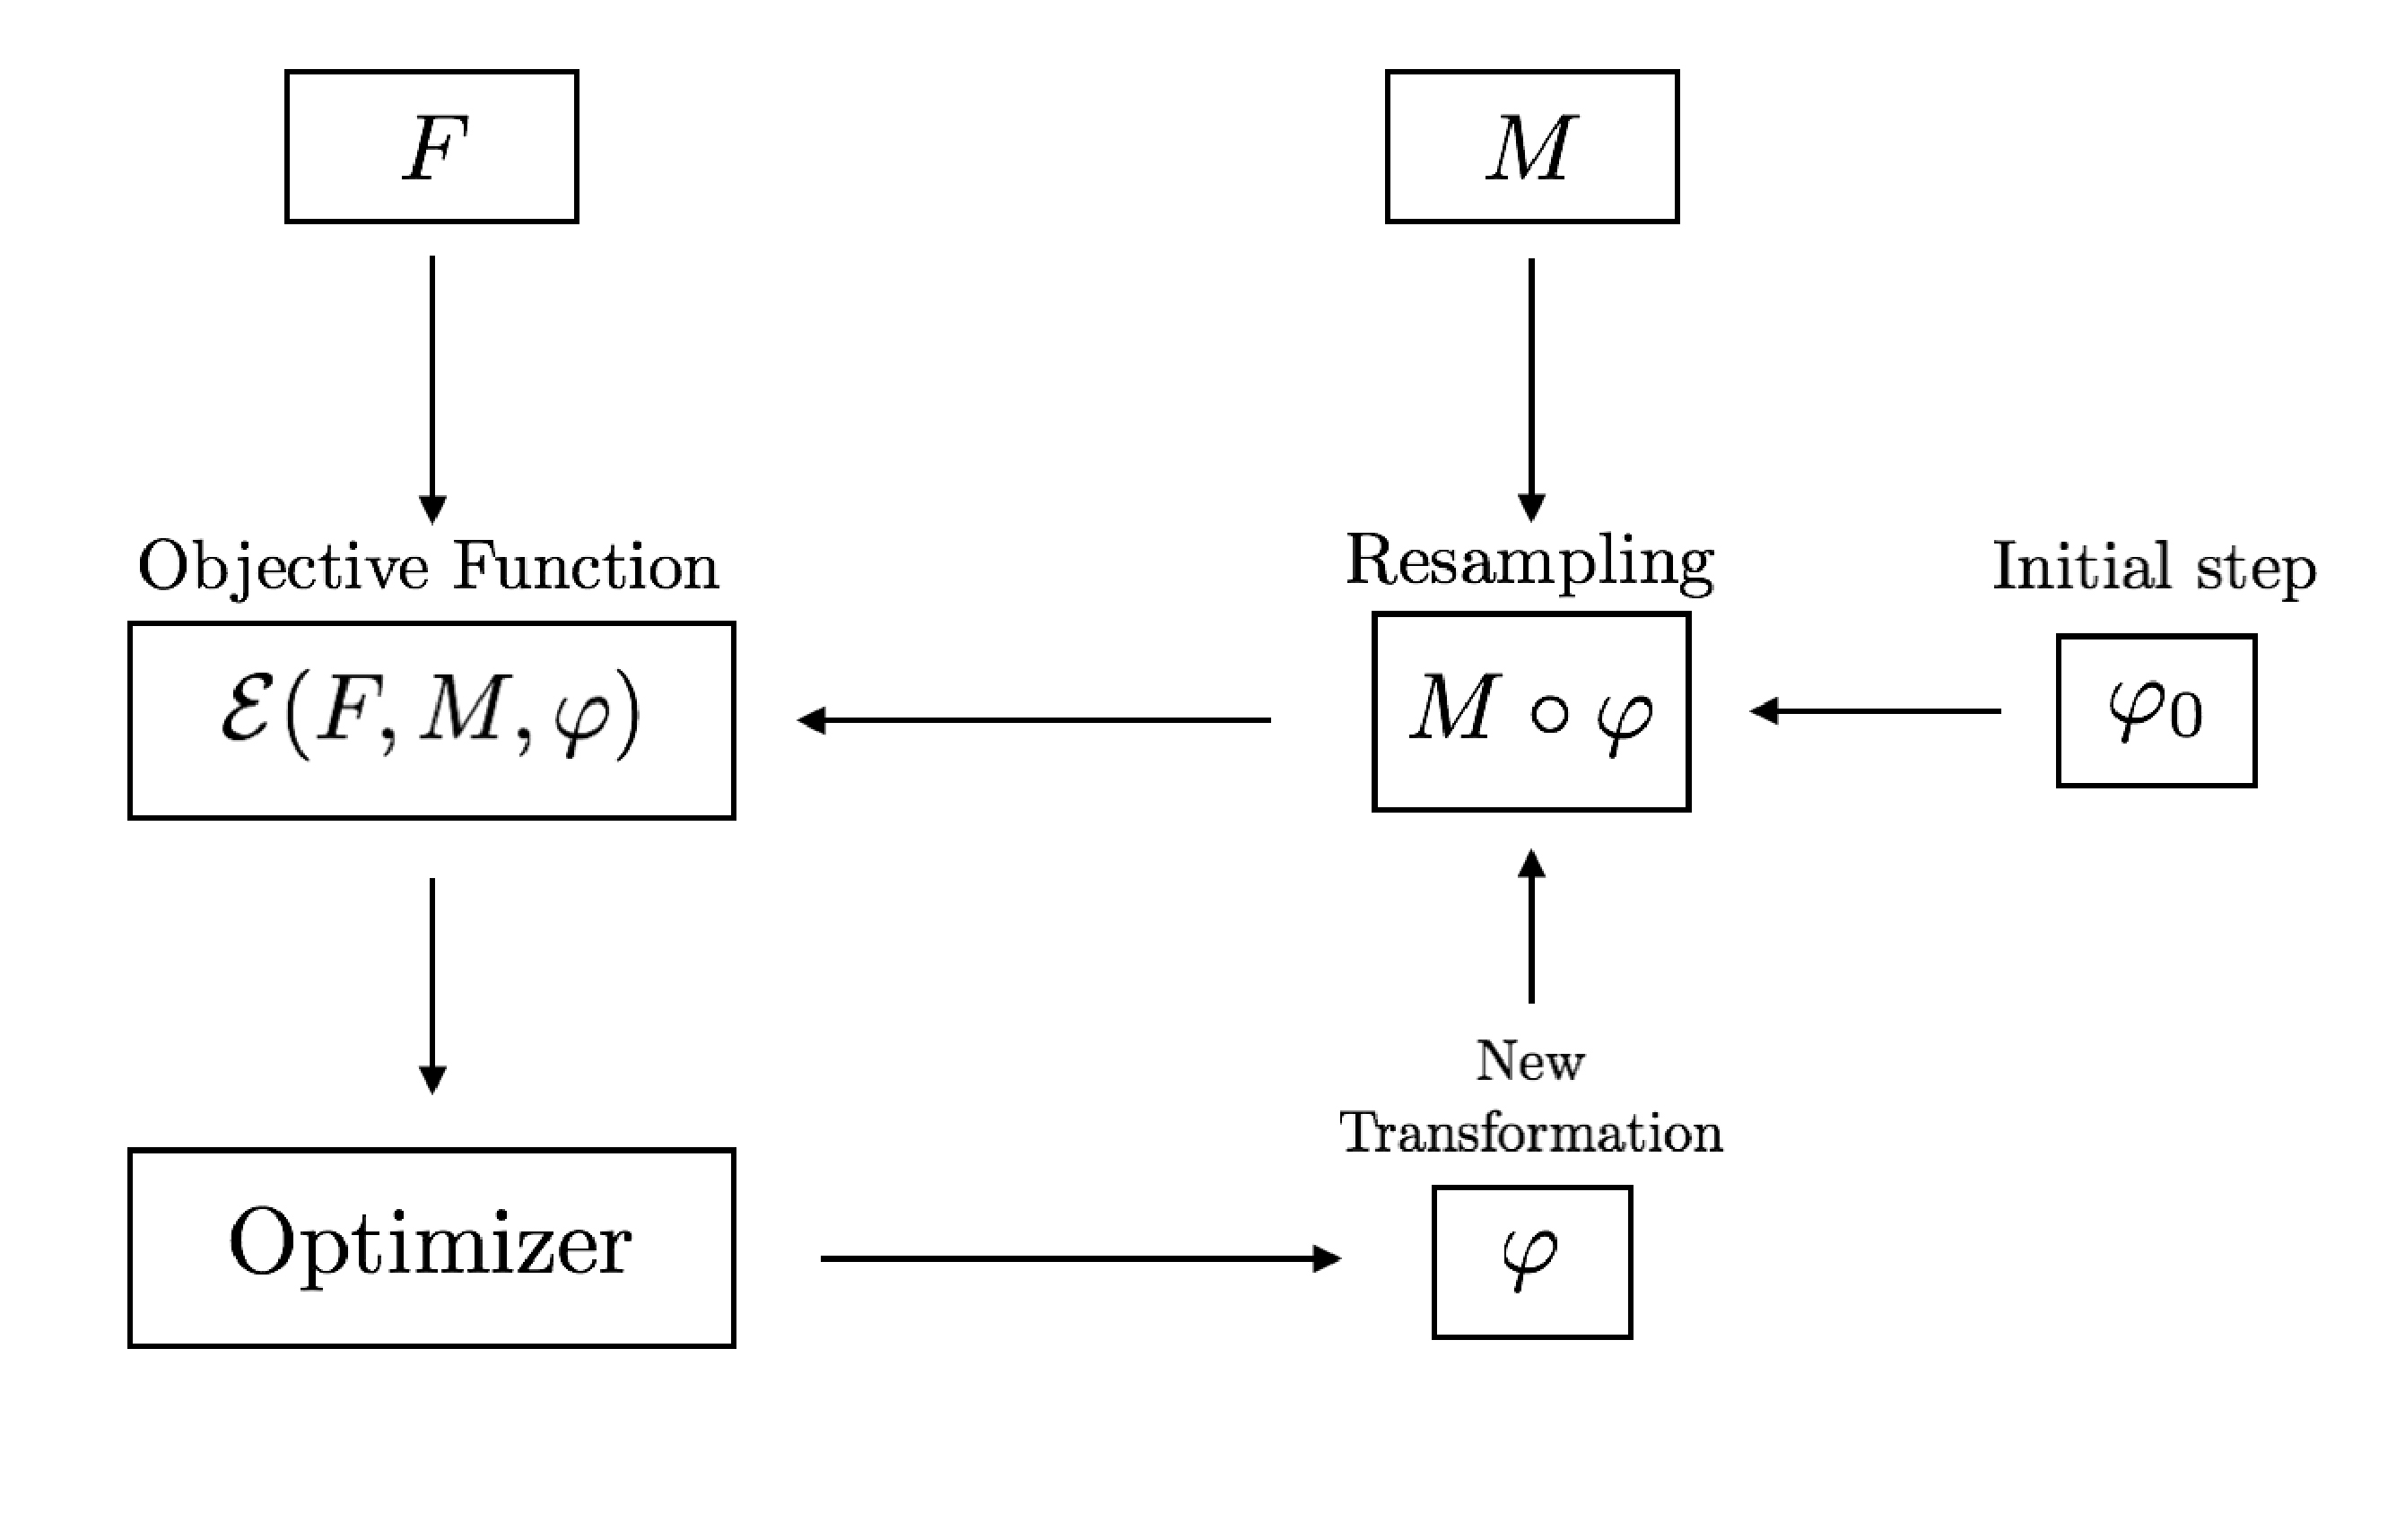
\includegraphics[scale=0.25]{figures/iterative_algorithm.pdf}
	\caption{Flowchart of the image registration framework.}
	\label{fig:iterative_algorithm_scheme}
\end{figure}
The flowchart of the framework is shown in figure \ref{fig:iterative_algorithm_scheme}: given a fixed image $F$, a moving image $M$ and an initial transformation $\varphi_0$, the warped image $M\circ\varphi_{0}$ is computed, and the 
energy function \ref{eq:general_cost_function} is optimized at each step by the algorithm. The resulting new transformation $\varphi$ takes the place of $\varphi_0$ for the subsequent steps.

Many of the available registration algorithms roughly follow this scheme, and the specific choice of the $5$ parameters involved provides a preliminary classification of the algorithm.
For further details see for example the recent surveys \cite{Sotiras:survey:13} and the less recent \cite{zitova2003image}. 

% % % % % % % % % % % % % % % % % % % % % % % % % % % % % % % % % % % % % %
% % SECTION
% % % % % % % % % % % % % % % % % % % % % % % % % % % % % % % % % % % % % %
\section{Diffeomorphisms in Medical Imaging Registration}

In any image registration algorithm, one of the most relevant feature is the choice of the family to whom the transformation belongs. This is as an important constraint that change according to the aim of the registration and to the nature of the objects represented by the images. 

If the algorithm is meant to model physical transformations that preserve distances, orientations and angles, then the set of transformations can be bonded to the group of rigid rotations and translations in three dimensions, $SE(3)$. The consequent registration algorithm, called \emph{rigid-registration algorithm}, will be suitable for example to compensate the motion in a rapid sequence of scans, or to investigate small differences that occurs in longitudinal scans.

If the algorithm is meant to model transformations that only preserves topology, then the transformations must allow more freedom than the one chosen for the rigid case. It is in this context that the mathematical objects of \emph{diffeomorphisms} are taken into account. These are defined as bijective differentiable maps with differentiable inverse, and are particularly well suited to model non-rigid deformations between images (for a  general introduction on diffeomorphisms see for example \cite{lee2012introduction}, \cite{arnold2006ordinary}). Consequent algorithms are called \emph{diffeomorphic registration algorithms}.

These algorithms, thanks to the property of invertibility and topology-preserving of the transformations involved, appears to be a natural choice to model organs' deformations and in many cases are the ideal candidate for the set of transformation in the registration framework. This is due to the fact that in longitudinal studies, anatomies are involved in a smooth process of modification over time that do not presume any breaking of topology. Also in most of the cross-sectional studies variations in the topology of the same organ in different patients are not expected. 

It is importance to notice that, when implemented in image registration algorithms, diffeomorphisms do not have only radically different results than the rigid body transformations: they also possess a different mathematical structure.

% % % % % % % % % % % % % % % % % % % % % % % % % % % % % % % % % % % % % %
% %  SUBSECTION
% % % % % % % % % % % % % % % % % % % % % % % % % % % % % % % % % % % % % %
\subsection{Utility and Liability of Diffeomorphisms}\label{se:diffe_util_and_liab}

On the algebraic side, the set of diffeomorphisms appears particularly interesting for their group structure and within their differentiable nature (see for example \cite{michor1980manifolds} and \cite{lempert1997problem}). They have also an infinite-dimensional structure of vector space, and their mathematical formalization as Lie group (so as differentiable manifold within a group structure, see \cite{warner}, \cite{lee2012introduction}) is an open field of research whose development has not yet reach a definitive formalization.

Attempt to provide some handles to the group of diffeomorphisms for easy manipulation was done for the first time in 1966 by Vladimir Arnold \cite{arnold1966geometrie} (consider also the equivalent \cite{arnold1998topological}, more readable for non-French speakers). To solve differential equation in hydrodynamic, the set of diffeomorphisms $\text{\emph{Diff}}$ is considered as a Lie group possessing a Lie algebra. This assumption is not formally followed in accordance to the problem-oriented nature of this paper. Subsequent steps in the exploration of the set of diffeomorphisms as a Lie group, and in the attempt of finding a formalization can be found in \cite{marsden1970hamiltonian, ebin1970groups, omori1970group, michor1980manifolds, leslie1983lie}. A state of the art of  infinite dimensional Lie group in early eighties can be found in \cite{Milnor:84:remarks}, while more recent results and applications on diffeomorphisms has been published in \cite{ovsienko1992integrals, bauer2010sobolev, schmid2010infinite,  bauer2011geodesic}.

Considering an infinite dimensional group as a differentiable manifold implies the idea of having each of its element in local correspondence with some generalized \lq\lq infinite-dimensional Euclidean\rq\rq\phantom{z}space. Attempt to set this correspondence showed that, the transition maps are smooth over the Banach spaces. This led to the idea of Banach Manifolds. It has been shown \cite{khesin2008geometry} that the group of diffeomorphisms defined as a manifold does not belongs to the category of Banach manifold but requires an even more general space on which the transition maps are smooth: the Frechet space. Here, important theorems from analysis, as the inverse function theorem, the Frobenius theorem, or the main results from the Lie group theory in a finite dimensional settings, as Lie correspondence theorems, do not holds anymore. 

These difficulties led some researchers in approaching the set of diffeomorphisms from other perspectives: 
for example, instead of treating $\text{\emph{Diff}}$ as a group equipped with differential structures, it is seen as a quotient of other well behaved group \cite{wojtynski1994one}. In other cases, as in \cite{marsden1970hamiltonian} first and in \cite{milnor1984remarks} later, Banach spaces are substituted with more general locally convex spaces to underpin the definition of smooth manifolds (an formal introduction to the infinite dimensional linear Lie groups, group of smooth maps and group of diffeomorphisms can be found in \cite{neeb2006infinite}).

For the medical imaging purposes, it is not necessary to consider the general theory of infinite dimensional manifolds. Keeping the initial Arnold's problem-oriented perspective, the interest is only toward the diffeomorphisms defined on a compact subset of $\mathbb{R}^d$. Without denying the importance of fundamentals and underestimating the doors research for generalized infinite dimensional Lie group may open, on the formal side we will approach the matter in as similar way of what has been done in set theory: we will use a \emph{naive approach} to infinite dimensional Lie group. Here the fundamental definition of infinite dimensional Lie group is a generalization of the finite dimensional case of matrices, and it is left more to the intuition than to a robust formalization. 

% % % % % % % % % % % % % % % % % % % % % % % % % % % % % % % % % % % % % %
% % % % % % % % % % % % % % % % % % % % % % % % % % % % % % % % % % % % % %
\subsection{State of the Art}\label{se:state_of_the_art}

In the development of diffeomorphic image registration, we can broadly identify some steps that led to the diffeomorphic demons and to the consequent concept of log-composition presented in this research:
\begin{enumerate}
	\item[1981-1996 $\triangleright$] The use of diffeomorphisms in medical image registration began from the research of a solution to a class partial differential equations: deformations are modeled as the consequent effect of two balancing forces applied to an elastic body \cite{Broit:1981} or to conserve the energy momentum \cite{christensen1996deformable}. In this early stage, diffeomorphisms are the domain of the solution of a set of differential equation, and are not considered with their Lie group structure.
	%
	\item[1998-2004 $\triangleright$] Based on the concept of attraction, the demons algorithm \cite{thirion1998image}, \cite{pennec1999understanding} proposes the computation of the transformation between images in an iterative framework, where the update of the transformation at each step is parametrized with a discrete vector field of independent vectors (or demons) that is optimized at each step. Each voxel of the moving image is considered within a vector that transforms it into a new position, according to the positions of the voxel of the same intensity in the fixed image. \\
	Here diffeomorphisms are not directly involved and the vectors at each voxel are independent elements. 
	In the same year of \cite{thirion1998image}, the utilization of diffeomorphism was taken into account in image matching and computational anatomy, not only as the set of solutions of some family of differential equations, but with its tangent space \cite{Dupuis:98:variationalproblems,  trouve1998diffeomorphisms, grenander1998computational}.
	%
	\item[2005-2006 $\triangleright$] In this period it has been proposed the Beg's version of Large Deformation Diffeomorphic Metric Mapping (called in this research Beg-LDDMM, to distinguish from others LDDMM versions) \cite{beg2005computing} for diffeomorphic image registration and the log-Euclidean framework \cite{arsigny2006statistics, Arsigny:MRM:06}  as an investigation of the tangent space to the Lie group of diffeomorphisms as a space where to perform statistics.
	The Beg-LDDMM utilizes in practice all of the opportunities provided by differential geometry in considering tangent vectors to the space of transformation in a framework for the computation of image registration. In this setting, the tangent vector field comes from the solution of the ODE that models the transformations and it consists of the set of the non-stationary vector field (also time varying vector field or TVVF). After the log-Euclidean framework aimed at the computation of statistics of diffeomorphisms, only the subset of the group of diffeomorphisms that are parametrized by stationary vector fields (also stationary velocity field or SFV) is taken into account for practical computations.
	%
	\item[2007-2013 $\triangleright$] The restriction to SVF was subsequently considered in some further improvements of Beg-LDDMM, as DARTEL \cite{Ashburner:07} and Stationary-LDDMM  \cite{hernandez2007registration}. 
	Log-Euclidean framework brought new life also to the demons algorithm, that, in 2007, become the diffeomorphic demons \cite{vercauteren2007non}.
	Subsequent approaches involving the symmetrization of the energy function and the use of a different measures of similarity (local correlation coefficient instead of $L^{2}$) are proposed in symmetric log-demons \cite{vercauteren08} and LCC-demons \cite{lorenzi2013lcc} respectively.
	
\end{enumerate}
\noindent
In the next section we will focus our attention on the diffeomorphic demons algorithm, as the starting point of the operation of log-composition, main subject of the following chapters.

% % % % % % % % % % % % % % % % % % % % % % % % % % % % % % % % % % % % % %
% % SUB SECTION
% % % % % % % % % % % % % % % % % % % % % % % % % % % % % % % % % % % % % %
\section{Demons Algorithms: From Classic to Diffeomorphic}

% classic demonclass
The first demons-based algorithm in image registration was proposed by \cite{thirion1998image} in analogy with the Maxwell's demon in thermodynamics. This early version - often called \emph{classic demons} - does not involves diffeomorphisms: the deformation is not bonded to any particular set of transformations and its smoothness is obtained with a Gaussian filter.

All the vectors applied to each voxel in the moving image are mutually independent, and are attracted by all of the voxels of the fixed image with similar intensity. The force of attraction are inspired by the optical flow equations \cite{horn1981determining}, and the algorithm works under the hypothesis that the intensity of a moving object is constant over time and it is therefore not robust to noise. 

The final deformation, solution of the registration problem is obtained composing at each step the previous transformation with an update. Indicating with $\varphi_{k}$ the deformation obtained at the beginning of the $k$-th iteration and with $\delta \varphi_{k}$ the update computed at the same step, they can be expressed as the addition between the identity and a displacement field $V$ or $\delta V$:
\begin{align*}
	\varphi_{k}(\mathbf{x}) &= \mathbf{x} + V_{k}(\mathbf{x}) \\ 
	\delta \varphi_{k}(\mathbf{x}) &= \mathbf{x} + \delta V_{k}(\mathbf{x}) 
\end{align*}
And with this notation the $k+1$-th deformation is computed by composition as:
\begin{align*}
\varphi_{k+1}(\mathbf{x})  :&= (\delta \varphi_{k}\circ \varphi_{k})(\mathbf{x}) \\
&= \mathbf{x} + \delta V_{k}(\mathbf{x}) + V_{k}(\mathbf{x} + \delta V_{k}(\mathbf{x}))
\end{align*}
Since the third addend is close to $V_{k}(\mathbf{x})$, many implementations - as for example the open-source Insight Segmentation and Registration Toolkit (ITK) \cite{yoo2002engineering} - consider by default only the sum between 
$ V_{k+1}$ and $V_{k}$ in the computation of the update:
\begin{align*}
\varphi_{k+1}(\mathbf{x})  :&= (\delta \varphi_{k} + \varphi_{k})(\mathbf{x}) \\
&= \mathbf{x} + V_{k}(\mathbf{x}) + \delta V_{k}(\mathbf{x})
\end{align*}
Demons algorithms with this implementation of the update are called \emph{additive demons}.

%PASHA
In \cite{cachier2003iconic} authors presents the PASHA demons as an extension of the classic demons, where a global energy function is considered and optimized according to an alternating minimization scheme. 
It is important to notice that again the PASHA algorithm does not involve any diffeomorphism, but it utilizes the framework presented in the previous section within maintaining the application of a Gaussian filter $G$ to smooth the transformations:
\begin{align*}
\varphi_{k+1}(\mathbf{x})  &:= G_{1}(\varphi_{k}(\mathbf{x}) + G_{2}(\delta \varphi_{k}(\mathbf{x}))
\end{align*}
% smoother as gaussian
In general, if $G_{1}$ is the identity the model is sometime called \emph{fluid}, while if $G_{2}$ is the identity is called \emph{elastic}.

Diffeomorphisms were introduced later within the demons algorithm (\emph{diffeomorphic demons} \cite{vercauteren2006robust}) after the presentation of the log-Euclidean framework \cite{Arsigny:MRM:06}. 
To each stationary velocity field $V \in \mathcal{V}(\Omega)$ is associated a diffeomorphisms $\varphi$ by the ODE $d\varphi /dt = V_{\varphi(t)} $, with the initial condition $\varphi(0) = \mathbf{x}$.\\
Using Lie theory, SVF are considered elements in the \emph{Lie algebra} - vector space defined by the differentiable vector field over $\Omega$, denoted with $\mathcal{V}(\Omega)$ or $\mathfrak{g}$ in Lie theory - while the set of diffeomorphisms defines a \emph{Lie group} - denoted with $\text{Diff}(\Omega)$ or with $\mathbb{G}$ -.

Roughly speaking, the Lie algebra $\mathcal{V}(\Omega)$ is the tangent space (as local linear approximation) to the Lie group $\text{Diff}(\Omega)$, and these two spaces are in local correspondence thanks to two functions: the \emph{Lie exponential} and the \emph{Lie logarithm}. \emph{Lie exponential} maps vector fields on the corresponding Lie group elements, while the \emph{Lie logarithm} - inverse of the Lie exponential under some condition, see \cite{do1976differential} or \cite{lee2012introduction} - maps each diffeomorphisms in the correspondent tangent vector field:
\begin{align*}
\varphi = \exp(V)  
\quad
V = \log(\varphi ) 
\qquad \qquad
\varphi  \in \mathbb{G}
\quad
V \in \mathfrak{g}
\end{align*}
In this settings, the update can not be computed simply with a sum of vector fields, since it must reflect the composition of the corresponding diffeomorphisms in the Lie group.

Several approaches have been presented to face the problem of the computation of the update. Diffeomorphic demons compute the transformation at each step of the iterative algorithm as the composition between the diffeomorphism $\varphi_{k}$ obtained at the previous step with the update $\delta V_{k}$, obtained with the optimization algorithm:
\begin{align*}
\varphi_{k + 1} := \varphi_{k}  \circ \exp(\delta V_{k})
\end{align*}
In a subsequent version, the log-demons \cite{vercauteren08}, the composition is performed in the tangent space toward exponential and logarithm functions
\begin{align}\label{eq:bch_problem}
V_{k + 1} := \log( \exp(V_{k})  \circ \exp(\delta V_{k}))
\end{align}
For this last computation, another theoretical element from the theory of Lie group has been utilized: the BCH formula. It provides the solution for $Z$ of the equation 
\begin{align*}
 \exp(Z) = \exp(X)\circ\exp(Y)
\end{align*}

As we will see in the subsequent sections, its solution involves an infinite series of nested Lie bracket that do not make its computation straightforward. 
To face the problem of its numerical approximation, whose solutions are utilized to solve \ref{eq:bch_problem}, we define in this thesis an inner binary operation called log-composition:
\begin{align*}
X \oplus Y := \log(\exp(X)\circ\exp( Y))
\qquad \qquad
\forall ~X, Y \in \mathfrak{g}
\end{align*}
That in the seminal paper about the computation of the coefficients of the BCH formula $\cite{dynkin1947calculation}$ appears indicated with $\Phi$.

The main aim of this research is to present a comparison between numerical methods for its computation.
Before presenting some details of the mathematical theory that underpins the numerical methods it is important to notice that the practical applications of the Log-composition do not impact only the update's composition in the log-demons.

% % % % % % % % % % % % % % % % % % % % % % % % % % % % % % % % % % % % % %
% % SECTION
% % % % % % % % % % % % % % % % % % % % % % % % % % % % % % % % % % % % % %
\subsection{Possible application of the Log-composition}
% why log composition:
In medical imaging there are several situations in which numerical methods and approximations passes through concepts equivalent to the log-composition.
 % where we can use the log composition
Its fast and accurate computation may therefore have an impact in the following $5$ situations:
\begin{enumerate}
	\item Symmetric diffeomorphic demons \cite{vercauteren08} - as introduced in equation \ref{eq:bch_problem}.
	\item Fast computation of the logarithm \cite{Bossa:08} - as discussed in chapter \ref{ch:log_algorithm}.
	\item Calculus on diffusion tensor \cite{Arsigny:MRM:06} - the log-composition appears as the dual operation of $\odot$ of the logarithmic multiplication for tensor defined at page 413. An approach to symmetric positive definite matrices that starts from the tangent space (where a metric can be directly computed without the application of the logarithm) may benefit of an accurate log-composition.  
	\item Image set classification \cite{huanglog} - as based on the log-euclidean metric on the group of symmetric positive definite matrices.
	\item Computation of the the discrete ladder for the parallel transport - in equation (2) of page $11$ fo the paper \cite{Lorenzi:discrete_ladders:14}, an equivalent of the log-composition is utilized to the computation of parallel transport. Reversing the procedure, parallel transport can be used for the computation of log-composition (as presented in \ref{se:parallel_transport}). Therefore any other improvement of the computation of the log-composition can be applied in this context and it provides immediate results to compute the parallel transport.
\end{enumerate}	
	
The next chapter is aimed to the formal definition of the log-composition, underpinned with the tools from differential geometry theory, and to present two new numerical technique for its computation.







%
%% % % % % % % % % % % % % % % % % % % % % % % % % % % % % % % % % % % % % %
%% % SUB SECTION
%% % % % % % % % % % % % % % % % % % % % % % % % % % % % % % % % % % % % % %
%\subsection{LDDMM: Classic, Shooting and Stationary}\label{se:intro_lddmm}
%
%As previously done in the elastic registration \cite{Broit:1981}, the LDDMM framework \cite{beg2005computing} originates by considering motion between images as the motion of a fluid, and utilizes ODE from fluid dynamics to compute the deformation between fixed and moving image. 
%% V
% A \emph{time varying vector field} (TVVF) is the continuously differentiable map defined as
% \begin{align*}
% 	V:[0,1] & \longrightarrow  \mathcal{V}(\Omega)\\
% 	t  &\longmapsto  V_{(t)}  : \Omega \longrightarrow   \mathbb{R}^{d} \\
% 	& \qquad \quad \quad ~~~\mathbf{x} \longmapsto V_{(t,\mathbf{x} )}
% \end{align*}
% % ODE
% Once initial conditions are given, at each TVVF, corresponds a unique time varying (or non-stationary) homomorphisms defined  by the following ODE 
% \begin{align}\label{eq:ode_phi_v}
% 	\frac{d\phi_{t} (\mathbf{x})}{dt} = V_{(t,\phi_{t} (\mathbf{x}) )}
% \end{align}
% % phi
% where the function $\phi$ is a path on the set of homeomorphisms  (continuous function from the background space $\Omega$ to itself with continuous inverse), indicated with $\text{Hom}(\Omega)$:
% \begin{align*}
% 	\phi : [0,1] & \longrightarrow  \text{Hom}(\Omega)\\
% 	t  &\longmapsto \phi_{t}  : \Omega \longrightarrow    \Omega \\
% 	& \qquad \quad \quad  \mathbf{x} \longmapsto \phi_{t}  (\mathbf{x} )
% \end{align*}
%%varphi
%The sought transformation $\varphi$ between fixed and moving images (such that it satisfies $ F\circ \varphi^{-1} \simeq M $), is modeled in the LDDMM as the solution of the equation \ref{eq:ode_phi_v} at time $1$. Using the fundamental theorem of calculus we obtain:
% \begin{align*}
% 	\varphi := \phi_{1} = \phi_{0} + \int_0^1 V_{(t,\phi_{t} (\mathbf{x}) )} dt
% \end{align*}
% % Orbits
%The set of homeomorphisms is taken into account since it can define a partition of the set of images into equivalence classes, as orbits of the action on the set of images from the background space $\mathcal{I}_{\Omega}$ (see for example \cite{artin2011algebra}, or \cite{trouve2005metamorphoses} for group action in computational anatomy). In other words, given a subgroup of homeomorphisms $\mathbb{G}\subseteq \text{Hom}(\Omega)$ and an image $F$, the orbit of the action of $\mathbb{G}$ over $F$, given by
%\begin{align*}
%\mathcal{O}_{\mathbb{G}}(F) = \{ F\circ \varphi^{-1} \mid \varphi \in \mathbb{G} \}
%\end{align*}
%consists in the set of the images having the same topology of $F$.
%
%%Diff, geodesics
%The model proposed in the LDDMM framework imposes a first constraint in considering $\mathbb{G}$ as the set of diffeomorphisms, and a second constraint considering $\phi_{t}$ as the shortest path between the identity function on $\mathbb{G}$ and $\varphi$. In this way the resulting vector field $V_{(t,\phi_{t} (\mathbf{x}))}$ is the one that minimize the distance $l$ between transformations:
%\begin{align*}
%\hat{l} = \inf_{V_{(t,\phi_{t} (\mathbf{x}))} ~ : ~ \dot{\phi_{t}} (\mathbf{x}) = V_{(t,\phi_{t} (\mathbf{x}))}  
%				       }
%	\int_{0}^{1} \euclideanMetric{V_{(t,\phi_{t} (\mathbf{x}))}}_{L^2}^{2}dt
%\end{align*}
%% Sim Reg - optimization function:
%For the similarity term the LDDMM uses the $L^{2}$ norm (see for example \cite{stein2009real}, chapter 4) between the moving image and the fixed image in the same orbit:
%\begin{align*}
%\text{Sim}(F,M,\varphi) = \frac{1}{\sigma^2}\euclideanMetric{F(\varphi^{-1})  - M  }_{L^{2}}^{2}
%\end{align*}
%while the regularization term is defined on the norm of the vector tangent to the transformation. Therefore, the optimization function is: 
%\begin{align*}
%\mathcal{E}(F, M, \varphi) 
%= 
%\frac{1}{\sigma^2}\euclideanMetric{F(\varphi^{-1})  - M  }_{L^{2}}^{2}
% +
%\int_0^1 \euclideanMetric{L V_{(t,\phi_{t} (\mathbf{x}))} }_{L^{2}}^{2} dt
%\end{align*}
%
%% discretization 
%As in many other implementation, also in the LDDMM the data structure utilized to store deformation fields are 5-dimensional matrices
%\begin{align}\label{eq:basic_data_structure}
%M = M(x_i,y_j,z_k,t,d) \qquad (i,j,k)\in L , ~~ t \in T  ~~ d = 1,2,3
%\end{align}
%where $(x_i,y_j,z_k)$ are discrete position of a lattice $L$ in the domain of the images, $t$ is the time parameter in a discretized domain $T$ and $d$ is index of the coordinate axis. So, the discretized \emph{tangent vector} $\mathbf{v}_{\tau}(x_i,y_j,z_k)$ at time $t$, has coordinates defined by
%\begin{align*}
%\mathbf{v}_{t}(x_i,y_j,z_k) = (M(x_i,y_j,z_k,t ,1), M(x_i,y_j,z_k,t,2), M(x_i,y_j,z_k,t ,3))
%\end{align*}
%% update 
%At the $k$-th step, the algorithm provides the 5-dim matrix $\mathbf{v}_{k}$ that is the approximation of the discretized time varying velocity fields $V_{(t,\phi_{t} (\mathbf{x}))}$. The update at each step is computed as
%\begin{align*}
%\mathbf{v}_{k+1} = \mathbf{v}_{k} - \epsilon \vec{\nabla} (\Delta\mathcal{E})
%\end{align*}
%where $\Delta\mathcal{E}$ is the discretized version of the energy function and $\epsilon$ is the gradient descent step size.
%
%% after LDDMM
%% shooting
%A direct upgrade of the classical LDDMM just introduced performs the optimization on the geodesic flows, defined by a set of Hamiltonian equation (Shooting LDDMM \cite{vialard2012diffeomorphic}). \\
%In this algorithm the iterative evolution of the deformation field, solution of the optimization algorithm, is regularized with the constraint imposed by an additional scalar field called \emph{initial momentum}. 
%%stationary: dartel and hernandez
%As proved by the authors, the evaluation of this constraint at each step provides geodesics flows of homeomorphisms, but it is computationally expensive. Taking advantages of the log-Euclidean framework presented in \cite{Arsigny:MRM:06}, a subsequent algorithm called DARTEL (Diffeomorphic Anatomical Registration using Exponentiated Lie Algebra \cite{Ashburner:07}) uses a constraint based on the stationarity of the involved velocity field. Instead of considering time varying velocity fields constrained by a set of Hamiltonian equations, the domain of vector field is reduced to the stationary velocity fields, whose consequence is a considerable reduction in the computational complexity. A similar algorithm, published in contemporary with DARTEL is \cite{hernandez2007registration}, based as well on the parametrization of geodesics path of diffeomorphisms with stationary velocity fields. 
%
%As happened in the case of the LDDMM, the log-Euclidean framework and the use of SVF had influenced also a second family of registration algorithm, called the \emph{demons algorithm}. In 2007, a new version of the demons, based on diffeomorphisms was proposed in \cite{vercauteren2006robust}. Aim of the next section is to introduce the diffeomorphic demons algorithm, second family of algorithm that exploit diffeomorphisms for the computation of the anatomical deformations.









